\documentclass[twoside]{book}

% Packages required by doxygen
\usepackage{fixltx2e}
\usepackage{calc}
\usepackage{doxygen}
\usepackage[export]{adjustbox} % also loads graphicx
\usepackage{graphicx}
\usepackage[utf8]{inputenc}
\usepackage{makeidx}
\usepackage{multicol}
\usepackage{multirow}
\PassOptionsToPackage{warn}{textcomp}
\usepackage{textcomp}
\usepackage[nointegrals]{wasysym}
\usepackage[table]{xcolor}

% Font selection
\usepackage[T1]{fontenc}
\usepackage[scaled=.90]{helvet}
\usepackage{courier}
\usepackage{amssymb}
\usepackage{sectsty}
\renewcommand{\familydefault}{\sfdefault}
\allsectionsfont{%
  \fontseries{bc}\selectfont%
  \color{darkgray}%
}
\renewcommand{\DoxyLabelFont}{%
  \fontseries{bc}\selectfont%
  \color{darkgray}%
}
\newcommand{\+}{\discretionary{\mbox{\scriptsize$\hookleftarrow$}}{}{}}

% Page & text layout
\usepackage{geometry}
\geometry{%
  a4paper,%
  top=2.5cm,%
  bottom=2.5cm,%
  left=2.5cm,%
  right=2.5cm%
}
\tolerance=750
\hfuzz=15pt
\hbadness=750
\setlength{\emergencystretch}{15pt}
\setlength{\parindent}{0cm}
\setlength{\parskip}{3ex plus 2ex minus 2ex}
\makeatletter
\renewcommand{\paragraph}{%
  \@startsection{paragraph}{4}{0ex}{-1.0ex}{1.0ex}{%
    \normalfont\normalsize\bfseries\SS@parafont%
  }%
}
\renewcommand{\subparagraph}{%
  \@startsection{subparagraph}{5}{0ex}{-1.0ex}{1.0ex}{%
    \normalfont\normalsize\bfseries\SS@subparafont%
  }%
}
\makeatother

% Headers & footers
\usepackage{fancyhdr}
\pagestyle{fancyplain}
\fancyhead[LE]{\fancyplain{}{\bfseries\thepage}}
\fancyhead[CE]{\fancyplain{}{}}
\fancyhead[RE]{\fancyplain{}{\bfseries\leftmark}}
\fancyhead[LO]{\fancyplain{}{\bfseries\rightmark}}
\fancyhead[CO]{\fancyplain{}{}}
\fancyhead[RO]{\fancyplain{}{\bfseries\thepage}}
\fancyfoot[LE]{\fancyplain{}{}}
\fancyfoot[CE]{\fancyplain{}{}}
\fancyfoot[RE]{\fancyplain{}{\bfseries\scriptsize Generated by Doxygen }}
\fancyfoot[LO]{\fancyplain{}{\bfseries\scriptsize Generated by Doxygen }}
\fancyfoot[CO]{\fancyplain{}{}}
\fancyfoot[RO]{\fancyplain{}{}}
\renewcommand{\footrulewidth}{0.4pt}
\renewcommand{\chaptermark}[1]{%
  \markboth{#1}{}%
}
\renewcommand{\sectionmark}[1]{%
  \markright{\thesection\ #1}%
}

% Indices & bibliography
\usepackage{natbib}
\usepackage[titles]{tocloft}
\setcounter{tocdepth}{3}
\setcounter{secnumdepth}{5}
\makeindex

% Hyperlinks (required, but should be loaded last)
\usepackage{ifpdf}
\ifpdf
  \usepackage[pdftex,pagebackref=true]{hyperref}
\else
  \usepackage[ps2pdf,pagebackref=true]{hyperref}
\fi
\hypersetup{%
  colorlinks=true,%
  linkcolor=blue,%
  citecolor=blue,%
  unicode%
}

% Custom commands
\newcommand{\clearemptydoublepage}{%
  \newpage{\pagestyle{empty}\cleardoublepage}%
}

\usepackage{caption}
\captionsetup{labelsep=space,justification=centering,font={bf},singlelinecheck=off,skip=4pt,position=top}

%===== C O N T E N T S =====

\begin{document}

% Titlepage & ToC
\hypersetup{pageanchor=false,
             bookmarksnumbered=true,
             pdfencoding=unicode
            }
\pagenumbering{alph}
\begin{titlepage}
\vspace*{7cm}
\begin{center}%
{\Large My Project \\[1ex]\large 1 }\\
\vspace*{1cm}
{\large Generated by Doxygen 1.8.13}\\
\end{center}
\end{titlepage}
\clearemptydoublepage
\pagenumbering{roman}
\tableofcontents
\clearemptydoublepage
\pagenumbering{arabic}
\hypersetup{pageanchor=true}

%--- Begin generated contents ---
\chapter{znc-\/self-\/msg}
\label{index}\hypertarget{index}{}Many irc clients that can connect to znc are not \textquotesingle{}irc3.\+0 capable\textquotesingle{}. As such, they do not have the ability to recieve their own messages. This module fixes that issue, giving self-\/message capability to {\itshape all} clients that connect to znc. For more info, please go to the \href{https://github.com/zwimer/znc-selfmsg/wiki}{\tt wiki}

\subsection*{Disclaimer}

This application is written for znc 1.\+6.\+4. Unfortunatly, the functions required for this to work for private channels do not yet exist. They will however be implemented in 1.\+7. Once 1.\+7 has been released and is stable, adding private message support should be trivial but unil then this will only work for public buffers.

\subsection*{Requirements}

This module requires znc 1.\+6.\+4. To build the \href{#documentation}{\tt documentation} for this module, Doxygen 1.\+8.\+3 is required. For installation, it is {\itshape strongly recommended} you have znc-\/buildmod unless you wish to compile and link this manually.

\subsection*{Installation Instructions}

First clone this repository Then git clone this repository 
\begin{DoxyCode}
git clone https://github.com/zwimer/znc-selfmsg
\end{DoxyCode}


Next cd into it and call znc-\/buildmod on selfmsg.\+cpp 
\begin{DoxyCode}
cd znc-selfmsg 
znc-buildmod selfmsg.cpp
\end{DoxyCode}


Finally, relocate the .so file znc-\/buildmod created to znc\textquotesingle{}s modules folder 
\begin{DoxyCode}
mv ./selfmsg.so ~/.znc/modules
\end{DoxyCode}


If this fails because no modules folder exists in $\sim$/.znc, simply create it with 
\begin{DoxyCode}
mkdir ~/.znc/modules
\end{DoxyCode}


\subsection*{Usage}

To use this module either load it with /\+Load\+Mod or via webadmin. After that it should work.

\subsection*{Documentation}

Additional documentation to each component of self\+\_\+msg.\+cpp is provided via Doxygen. To generate this documentation, from the znc-\/selfmsg directory, run the following 
\begin{DoxyCode}
doxygen Doxyfile
\end{DoxyCode}


The documentation \textquotesingle{}index.\+html\textquotesingle{} is located within Documentation/html/ 
\chapter{Namespace Index}
\section{Namespace List}
Here is a list of all documented namespaces with brief descriptions\+:\begin{DoxyCompactList}
\item\contentsline{section}{\hyperlink{namespace_s_m_h}{S\+MH} \\*A namespace to hold helper classes of \hyperlink{class_self_msg}{Self\+Msg} }{\pageref{namespace_s_m_h}}{}
\end{DoxyCompactList}

\chapter{Hierarchical Index}
\section{Class Hierarchy}
This inheritance list is sorted roughly, but not completely, alphabetically\+:\begin{DoxyCompactList}
\item C\+Module\begin{DoxyCompactList}
\item \contentsline{section}{Self\+Msg}{\pageref{class_self_msg}}{}
\end{DoxyCompactList}
\item \contentsline{section}{S\+MH\+:\+:Msg}{\pageref{struct_s_m_h_1_1_msg}}{}
\item \contentsline{section}{S\+MH\+:\+:Msg\+Compare}{\pageref{struct_s_m_h_1_1_msg_compare}}{}
\end{DoxyCompactList}

\chapter{Class Index}
\section{Class List}
Here are the classes, structs, unions and interfaces with brief descriptions\+:\begin{DoxyCompactList}
\item\contentsline{section}{\hyperlink{struct_s_m_h_1_1_msg}{S\+M\+H\+::\+Msg} \\*Represents a message }{\pageref{struct_s_m_h_1_1_msg}}{}
\item\contentsline{section}{\hyperlink{struct_s_m_h_1_1_msg_compare}{S\+M\+H\+::\+Msg\+Compare} \\*A comparator for \hyperlink{struct_s_m_h_1_1_msg}{Msg} }{\pageref{struct_s_m_h_1_1_msg_compare}}{}
\item\contentsline{section}{\hyperlink{class_self_msg}{Self\+Msg} \\*A znc module that allows one to receive their own messages }{\pageref{class_self_msg}}{}
\end{DoxyCompactList}

\chapter{Namespace Documentation}
\hypertarget{namespace_s_m_h}{}\section{S\+MH Namespace Reference}
\label{namespace_s_m_h}\index{S\+MH@{S\+MH}}


A namespace to hold helper classes of \hyperlink{class_self_msg}{Self\+Msg}.  


\subsection*{Classes}
\begin{DoxyCompactItemize}
\item 
struct \hyperlink{struct_s_m_h_1_1_msg}{Msg}
\begin{DoxyCompactList}\small\item\em Represents a message. \end{DoxyCompactList}\item 
struct \hyperlink{struct_s_m_h_1_1_msg_compare}{Msg\+Compare}
\begin{DoxyCompactList}\small\item\em A comparator for \hyperlink{struct_s_m_h_1_1_msg}{Msg}. \end{DoxyCompactList}\end{DoxyCompactItemize}
\subsection*{Typedefs}
\begin{DoxyCompactItemize}
\item 
typedef std\+::priority\+\_\+queue$<$ \hyperlink{struct_s_m_h_1_1_msg}{Msg}, std\+::vector$<$ \hyperlink{struct_s_m_h_1_1_msg}{Msg} $>$, \hyperlink{struct_s_m_h_1_1_msg_compare}{Msg\+Compare} $>$ \hyperlink{namespace_s_m_h_a577a58a147f501590720badab28c2c98}{Msg\+List}
\begin{DoxyCompactList}\small\item\em Msg\+Line is a priority queue of Msgs sorted via \hyperlink{struct_s_m_h_1_1_msg_compare}{Msg\+Compare}. \end{DoxyCompactList}\end{DoxyCompactItemize}


\subsection{Detailed Description}
A namespace to hold helper classes of \hyperlink{class_self_msg}{Self\+Msg}. 

Don\textquotesingle{}t pollute the global namespace with these classes. Instead, put them into a namespace. \hyperlink{namespace_s_m_h}{S\+MH} stands for Self \hyperlink{struct_s_m_h_1_1_msg}{Msg} Helpers. 

\subsection{Typedef Documentation}
\mbox{\Hypertarget{namespace_s_m_h_a577a58a147f501590720badab28c2c98}\label{namespace_s_m_h_a577a58a147f501590720badab28c2c98}} 
\index{S\+MH@{S\+MH}!Msg\+List@{Msg\+List}}
\index{Msg\+List@{Msg\+List}!S\+MH@{S\+MH}}
\subsubsection{\texorpdfstring{Msg\+List}{MsgList}}
{\footnotesize\ttfamily typedef std\+::priority\+\_\+queue$<$ \hyperlink{struct_s_m_h_1_1_msg}{Msg}, std\+::vector$<$\hyperlink{struct_s_m_h_1_1_msg}{Msg}$>$, \hyperlink{struct_s_m_h_1_1_msg_compare}{Msg\+Compare} $>$ \hyperlink{namespace_s_m_h_a577a58a147f501590720badab28c2c98}{S\+M\+H\+::\+Msg\+List}}



Msg\+Line is a priority queue of Msgs sorted via \hyperlink{struct_s_m_h_1_1_msg_compare}{Msg\+Compare}. 

The queue is stored via a vector 
\chapter{Class Documentation}
\hypertarget{struct_s_m_h_1_1_msg}{}\section{S\+MH\+:\+:Msg Struct Reference}
\label{struct_s_m_h_1_1_msg}\index{S\+M\+H\+::\+Msg@{S\+M\+H\+::\+Msg}}


Represents a message.  


\subsection*{Public Member Functions}
\begin{DoxyCompactItemize}
\item 
\hyperlink{struct_s_m_h_1_1_msg_a8c0752c26661975e08bdf6321eeea6b5}{Msg} (const timeval \&whn, const C\+String wht)
\begin{DoxyCompactList}\small\item\em Constructor. \end{DoxyCompactList}\item 
\mbox{\Hypertarget{struct_s_m_h_1_1_msg_a551b4ddc00b63deeda549586a8f9813a}\label{struct_s_m_h_1_1_msg_a551b4ddc00b63deeda549586a8f9813a}} 
\hyperlink{struct_s_m_h_1_1_msg_a551b4ddc00b63deeda549586a8f9813a}{Msg} (const timeval \&whn, const C\+String wht, const C\+String \&fmt)
\begin{DoxyCompactList}\small\item\em Constructor. \end{DoxyCompactList}\end{DoxyCompactItemize}
\subsection*{Public Attributes}
\begin{DoxyCompactItemize}
\item 
\mbox{\Hypertarget{struct_s_m_h_1_1_msg_a4664e37839bff3c5ad44862d3da0baa5}\label{struct_s_m_h_1_1_msg_a4664e37839bff3c5ad44862d3da0baa5}} 
timeval \hyperlink{struct_s_m_h_1_1_msg_a4664e37839bff3c5ad44862d3da0baa5}{when}
\begin{DoxyCompactList}\small\item\em When the message was sent. \end{DoxyCompactList}\item 
\mbox{\Hypertarget{struct_s_m_h_1_1_msg_afd60c6f95937d6ace7c19d08d56d8967}\label{struct_s_m_h_1_1_msg_afd60c6f95937d6ace7c19d08d56d8967}} 
C\+String \hyperlink{struct_s_m_h_1_1_msg_afd60c6f95937d6ace7c19d08d56d8967}{what}
\begin{DoxyCompactList}\small\item\em The message. \end{DoxyCompactList}\item 
\mbox{\Hypertarget{struct_s_m_h_1_1_msg_adb69dae7cbf7847d8b317c62dca88168}\label{struct_s_m_h_1_1_msg_adb69dae7cbf7847d8b317c62dca88168}} 
C\+String \hyperlink{struct_s_m_h_1_1_msg_adb69dae7cbf7847d8b317c62dca88168}{format}
\begin{DoxyCompactList}\small\item\em The format of the message. \end{DoxyCompactList}\end{DoxyCompactItemize}


\subsection{Detailed Description}
Represents a message. 

This struct contains a message, its format, and when it was sent 

\subsection{Constructor \& Destructor Documentation}
\mbox{\Hypertarget{struct_s_m_h_1_1_msg_a8c0752c26661975e08bdf6321eeea6b5}\label{struct_s_m_h_1_1_msg_a8c0752c26661975e08bdf6321eeea6b5}} 
\index{S\+M\+H\+::\+Msg@{S\+M\+H\+::\+Msg}!Msg@{Msg}}
\index{Msg@{Msg}!S\+M\+H\+::\+Msg@{S\+M\+H\+::\+Msg}}
\subsubsection{\texorpdfstring{Msg()}{Msg()}}
{\footnotesize\ttfamily S\+M\+H\+::\+Msg\+::\+Msg (\begin{DoxyParamCaption}\item[{const timeval \&}]{whn,  }\item[{const C\+String}]{wht }\end{DoxyParamCaption})\hspace{0.3cm}{\ttfamily [inline]}}



Constructor. 

This constructor takes in a timeval and message and creates the \hyperlink{struct_s_m_h_1_1_msg}{Msg} from them. This constructor leaves the format blank 

The documentation for this struct was generated from the following file\+:\begin{DoxyCompactItemize}
\item 
self\+\_\+msg.\+cpp\end{DoxyCompactItemize}

\hypertarget{struct_s_m_h_1_1_msg_compare}{}\section{S\+MH\+:\+:Msg\+Compare Struct Reference}
\label{struct_s_m_h_1_1_msg_compare}\index{S\+M\+H\+::\+Msg\+Compare@{S\+M\+H\+::\+Msg\+Compare}}


A comparator for \hyperlink{struct_s_m_h_1_1_msg}{Msg}.  


\subsection*{Public Member Functions}
\begin{DoxyCompactItemize}
\item 
bool \hyperlink{struct_s_m_h_1_1_msg_compare_afa4a56eba642be97adc3af0665588479}{operator()} (const \hyperlink{struct_s_m_h_1_1_msg}{Msg} \&a, const \hyperlink{struct_s_m_h_1_1_msg}{Msg} \&b)
\begin{DoxyCompactList}\small\item\em Compares two messages. \end{DoxyCompactList}\end{DoxyCompactItemize}


\subsection{Detailed Description}
A comparator for \hyperlink{struct_s_m_h_1_1_msg}{Msg}. 

\subsection{Member Function Documentation}
\mbox{\Hypertarget{struct_s_m_h_1_1_msg_compare_afa4a56eba642be97adc3af0665588479}\label{struct_s_m_h_1_1_msg_compare_afa4a56eba642be97adc3af0665588479}} 
\index{S\+M\+H\+::\+Msg\+Compare@{S\+M\+H\+::\+Msg\+Compare}!operator()@{operator()}}
\index{operator()@{operator()}!S\+M\+H\+::\+Msg\+Compare@{S\+M\+H\+::\+Msg\+Compare}}
\subsubsection{\texorpdfstring{operator()()}{operator()()}}
{\footnotesize\ttfamily bool S\+M\+H\+::\+Msg\+Compare\+::operator() (\begin{DoxyParamCaption}\item[{const \hyperlink{struct_s_m_h_1_1_msg}{Msg} \&}]{a,  }\item[{const \hyperlink{struct_s_m_h_1_1_msg}{Msg} \&}]{b }\end{DoxyParamCaption})\hspace{0.3cm}{\ttfamily [inline]}}



Compares two messages. 

Returns true if all bits in a are 0, false if all bits in b are 0. Otherwise, return a.\+when $>$ b.\+when 

The documentation for this struct was generated from the following file\+:\begin{DoxyCompactItemize}
\item 
self\+\_\+msg.\+cpp\end{DoxyCompactItemize}

\hypertarget{class_self_msg}{}\section{Self\+Msg Class Reference}
\label{class_self_msg}\index{Self\+Msg@{Self\+Msg}}


A znc module that allows one to receive their own messages.  


Inheritance diagram for Self\+Msg\+:\begin{figure}[H]
\begin{center}
\leavevmode
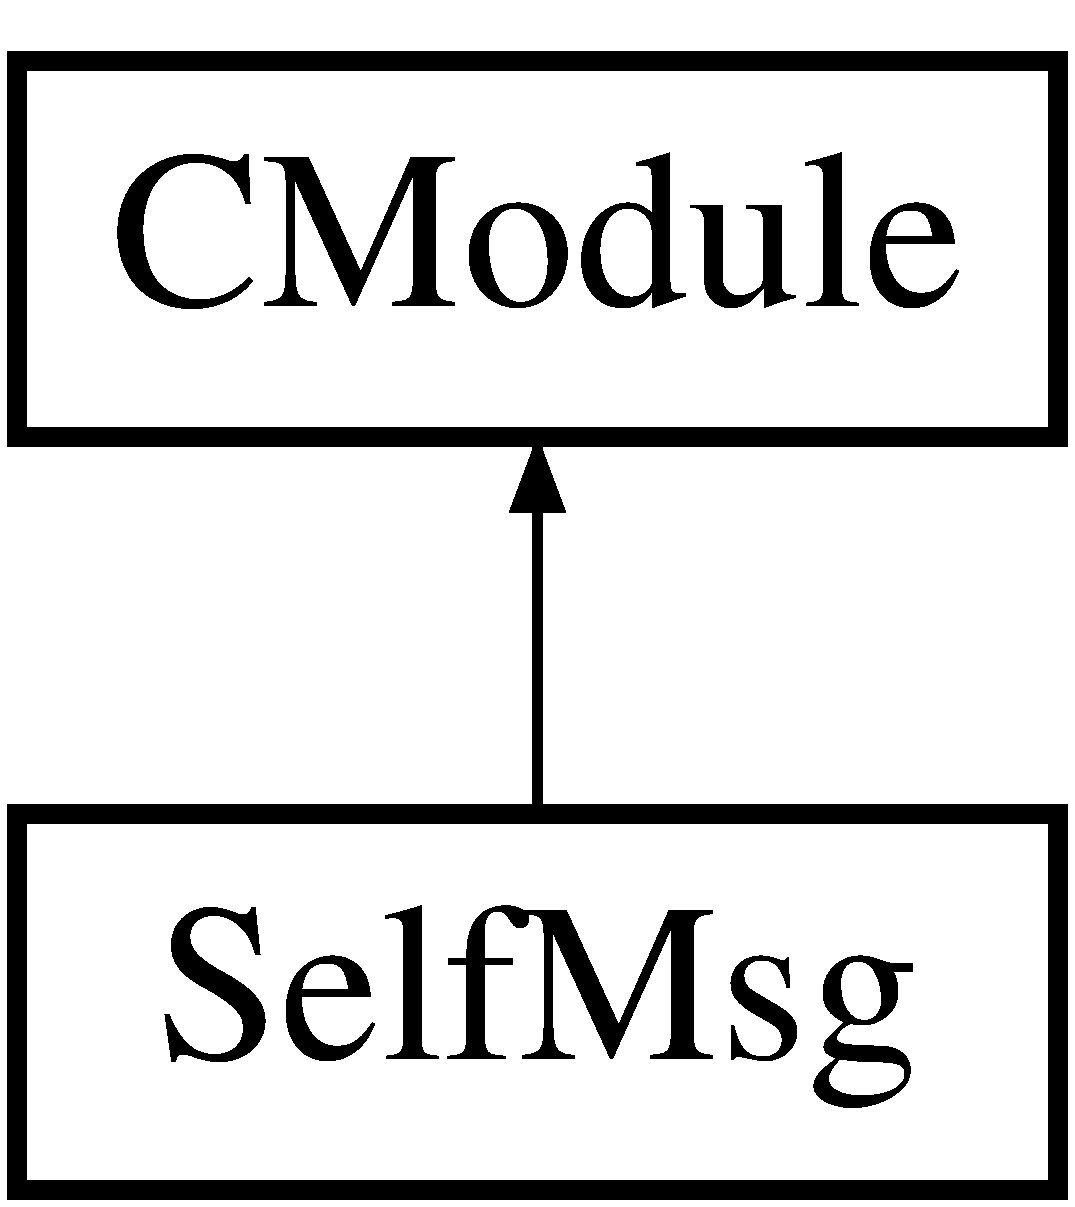
\includegraphics[height=2.000000cm]{class_self_msg}
\end{center}
\end{figure}
\subsection*{Public Member Functions}
\begin{DoxyCompactItemize}
\item 
\hyperlink{class_self_msg_a7eb533ec01cd81c8907fcf3a0ebd078e}{M\+O\+D\+C\+O\+N\+S\+T\+R\+U\+C\+T\+OR} (\hyperlink{class_self_msg}{Self\+Msg})
\begin{DoxyCompactList}\small\item\em Constructor. \end{DoxyCompactList}\item 
\hyperlink{class_self_msg_a7febe41f96890d89051a91840da84fab}{$\sim$\+Self\+Msg} () override
\begin{DoxyCompactList}\small\item\em Destructor. \end{DoxyCompactList}\item 
bool \hyperlink{class_self_msg_a59bd01047737a3b30ae430fc3612653d}{On\+Boot} () override
\begin{DoxyCompactList}\small\item\em Called when znc is first turned on. \end{DoxyCompactList}\item 
E\+Mod\+Ret \hyperlink{class_self_msg_ae86a578c56e20230f89d776e02b089d5}{On\+User\+Msg} (C\+String \&s\+Target, C\+String \&s\+Message) override
\begin{DoxyCompactList}\small\item\em Read every message the user sends. \end{DoxyCompactList}\item 
E\+Mod\+Ret \hyperlink{class_self_msg_a8c7c5d393c196048cd51b63bc8ba59b1}{On\+Chan\+Buffer\+Starting} (C\+Chan \&ch, C\+Client \&cli) override
\begin{DoxyCompactList}\small\item\em Alter the buffer being sent to the user. \end{DoxyCompactList}\end{DoxyCompactItemize}
\subsection*{Protected Attributes}
\begin{DoxyCompactItemize}
\item 
std\+::map$<$ C\+String, \hyperlink{namespace_s_m_h_a577a58a147f501590720badab28c2c98}{S\+M\+H\+::\+Msg\+List} $>$ \hyperlink{class_self_msg_ae2dc542caa1a3f5ae45e6de96d37cb22}{sent}
\begin{DoxyCompactList}\small\item\em Store each messages the user sent to who. \end{DoxyCompactList}\end{DoxyCompactItemize}


\subsection{Detailed Description}
A znc module that allows one to receive their own messages. 

This module will record all messages the user sends. When the user next connects to znc and requests their buffer, this module will add the user\textquotesingle{}s messages to the buffer they receive. 

\subsection{Constructor \& Destructor Documentation}
\mbox{\Hypertarget{class_self_msg_a7febe41f96890d89051a91840da84fab}\label{class_self_msg_a7febe41f96890d89051a91840da84fab}} 
\index{Self\+Msg@{Self\+Msg}!````~Self\+Msg@{$\sim$\+Self\+Msg}}
\index{````~Self\+Msg@{$\sim$\+Self\+Msg}!Self\+Msg@{Self\+Msg}}
\subsubsection{\texorpdfstring{$\sim$\+Self\+Msg()}{~SelfMsg()}}
{\footnotesize\ttfamily Self\+Msg\+::$\sim$\+Self\+Msg (\begin{DoxyParamCaption}{ }\end{DoxyParamCaption})\hspace{0.3cm}{\ttfamily [inline]}, {\ttfamily [override]}}



Destructor. 

Inform the user that this module has been unloaded 

\subsection{Member Function Documentation}
\mbox{\Hypertarget{class_self_msg_a7eb533ec01cd81c8907fcf3a0ebd078e}\label{class_self_msg_a7eb533ec01cd81c8907fcf3a0ebd078e}} 
\index{Self\+Msg@{Self\+Msg}!M\+O\+D\+C\+O\+N\+S\+T\+R\+U\+C\+T\+OR@{M\+O\+D\+C\+O\+N\+S\+T\+R\+U\+C\+T\+OR}}
\index{M\+O\+D\+C\+O\+N\+S\+T\+R\+U\+C\+T\+OR@{M\+O\+D\+C\+O\+N\+S\+T\+R\+U\+C\+T\+OR}!Self\+Msg@{Self\+Msg}}
\subsubsection{\texorpdfstring{M\+O\+D\+C\+O\+N\+S\+T\+R\+U\+C\+T\+O\+R()}{MODCONSTRUCTOR()}}
{\footnotesize\ttfamily Self\+Msg\+::\+M\+O\+D\+C\+O\+N\+S\+T\+R\+U\+C\+T\+OR (\begin{DoxyParamCaption}\item[{\hyperlink{class_self_msg}{Self\+Msg}}]{ }\end{DoxyParamCaption})\hspace{0.3cm}{\ttfamily [inline]}}



Constructor. 

The normal mod constructor \mbox{\Hypertarget{class_self_msg_a59bd01047737a3b30ae430fc3612653d}\label{class_self_msg_a59bd01047737a3b30ae430fc3612653d}} 
\index{Self\+Msg@{Self\+Msg}!On\+Boot@{On\+Boot}}
\index{On\+Boot@{On\+Boot}!Self\+Msg@{Self\+Msg}}
\subsubsection{\texorpdfstring{On\+Boot()}{OnBoot()}}
{\footnotesize\ttfamily bool Self\+Msg\+::\+On\+Boot (\begin{DoxyParamCaption}{ }\end{DoxyParamCaption})\hspace{0.3cm}{\ttfamily [override]}}



Called when znc is first turned on. 

Does nothing but override Module\textquotesingle{}s on boot function \mbox{\Hypertarget{class_self_msg_a8c7c5d393c196048cd51b63bc8ba59b1}\label{class_self_msg_a8c7c5d393c196048cd51b63bc8ba59b1}} 
\index{Self\+Msg@{Self\+Msg}!On\+Chan\+Buffer\+Starting@{On\+Chan\+Buffer\+Starting}}
\index{On\+Chan\+Buffer\+Starting@{On\+Chan\+Buffer\+Starting}!Self\+Msg@{Self\+Msg}}
\subsubsection{\texorpdfstring{On\+Chan\+Buffer\+Starting()}{OnChanBufferStarting()}}
{\footnotesize\ttfamily Self\+Msg\+::\+E\+Mod\+Ret Self\+Msg\+::\+On\+Chan\+Buffer\+Starting (\begin{DoxyParamCaption}\item[{C\+Chan \&}]{ch,  }\item[{C\+Client \&}]{cli }\end{DoxyParamCaption})\hspace{0.3cm}{\ttfamily [override]}}



Alter the buffer being sent to the user. 

This function intercepts the buffer being sent to the user. It then inserts each message the user sent into the buffer and finally clears the \textquotesingle{}sent\textquotesingle{} map. \mbox{\Hypertarget{class_self_msg_ae86a578c56e20230f89d776e02b089d5}\label{class_self_msg_ae86a578c56e20230f89d776e02b089d5}} 
\index{Self\+Msg@{Self\+Msg}!On\+User\+Msg@{On\+User\+Msg}}
\index{On\+User\+Msg@{On\+User\+Msg}!Self\+Msg@{Self\+Msg}}
\subsubsection{\texorpdfstring{On\+User\+Msg()}{OnUserMsg()}}
{\footnotesize\ttfamily Self\+Msg\+::\+E\+Mod\+Ret Self\+Msg\+::\+On\+User\+Msg (\begin{DoxyParamCaption}\item[{C\+String \&}]{s\+Target,  }\item[{C\+String \&}]{s\+Message }\end{DoxyParamCaption})\hspace{0.3cm}{\ttfamily [override]}}



Read every message the user sends. 

This function is called whenever the user sends a message. This function records each messages, relevant information, then stores it in the \textquotesingle{}sent\textquotesingle{} map 

\subsection{Member Data Documentation}
\mbox{\Hypertarget{class_self_msg_ae2dc542caa1a3f5ae45e6de96d37cb22}\label{class_self_msg_ae2dc542caa1a3f5ae45e6de96d37cb22}} 
\index{Self\+Msg@{Self\+Msg}!sent@{sent}}
\index{sent@{sent}!Self\+Msg@{Self\+Msg}}
\subsubsection{\texorpdfstring{sent}{sent}}
{\footnotesize\ttfamily std\+::map$<$ C\+String, \hyperlink{namespace_s_m_h_a577a58a147f501590720badab28c2c98}{S\+M\+H\+::\+Msg\+List} $>$ Self\+Msg\+::sent\hspace{0.3cm}{\ttfamily [protected]}}



Store each messages the user sent to who. 

This map has C\+String key denoting who each message was sent to. The value in the map is a list of messages sorted by when each message was sent. This map will hold all messages that must be added to the buffer when it is next intercepted. 

The documentation for this class was generated from the following file\+:\begin{DoxyCompactItemize}
\item 
self\+\_\+msg.\+cpp\end{DoxyCompactItemize}

%--- End generated contents ---

% Index
\backmatter
\newpage
\phantomsection
\clearemptydoublepage
\addcontentsline{toc}{chapter}{Index}
\printindex

\end{document}
